\section{Our Softmax Model}
\addcontentsline{toc}{section}{Our Softmax Model}
\label{sec:softmax-model}

For training the Softmax model on species classification, we decided to use all available training images. For Softmax standards, 51000 images are not that many. This is why we decided for train/validation/test split of $0.8$/$0.1$/$0.1$. \\
Since we wanted to train, validate and evaluate or model on predicting all 30 species, we wanted to have at least one image of every species present in every dataset. To achieve this, we used the \hyperref[subsubsec:smart-batches]{Smart Batches Algorithm}, simply because it likely to create such a split. \\
We called all functions with different seeds and quickly found the first valid candidate "$5$", which we then used for all our Softmax models.

\subsection{Configurations and Hyperparameters}
We loaded all architectures with the \textit{include\_top} setting as \textit{false} and set \textit{pooling} to \textit{max}. We then simply put a dense layer with 30 neurons for the species and a Softmax activation function on top. We choose \textit{Adam} as an optimizer with a \textit{learning rate} of $0.001$ and set \textit{Categorical Cross Entropy} loss. \\
Nothing special - pretty standard image classification settings.

\subsection{Evaluation}
\subsubsection{ImageNet vs Random Weights}
We first wanted to test whether loading our models with weights, which where pretrained on the ImageNet dataset, would lead to a faster convergence. To do this, we trained a ResNet50 for 10 epochs each. Once with the pretrained ImageNet weights and once with randomly initialized weights. The ImageNet weights beat the other in every metric. \\

\begin{figure}[ht] 
        \centering 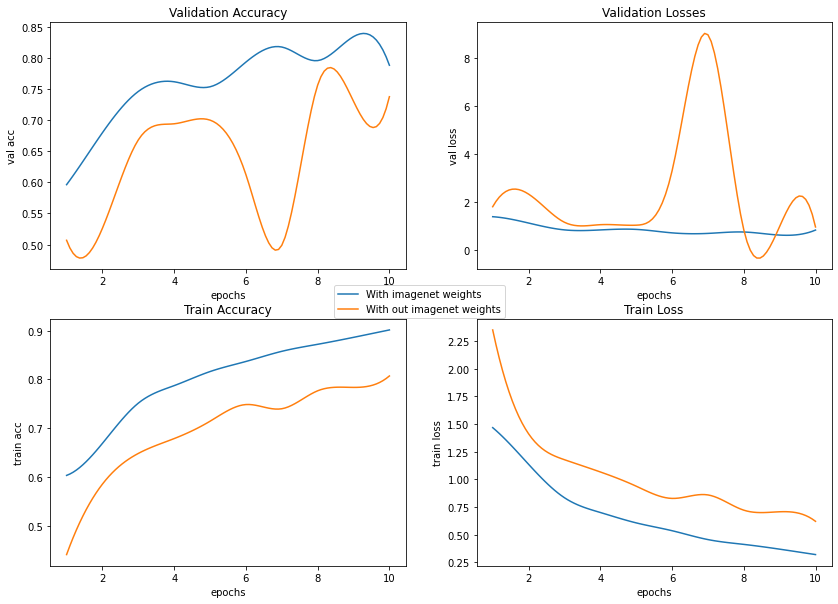
\includegraphics[width=1\columnwidth]{figures/comparison_softmax.png}
        \caption{\label{fig:comparison-softmax} ImageNet vs random performance.}
\end{figure}

\noindent Because of this, we then decided stick to models with ImageNet weights for our further analysis.

\subsubsection{Comparing CNN architectures}
Further, we test the performance of several CNNs. As mentioned in \hyperref[subsec:cnn]{CNN architecture}, we do not want too many parameters so we could still train them locally. We tested all architectures for 10-15 epochs. \\

\noindent These were the results:

\begin{table}[ht]
\begin{tabular}{ c c c c c }
  \hline
    \(Architectures\) &  \(ACC_{10}\) & \(s/epoch\) & \(ACC_{10}\)/time \\ \hline \hline
  ResNet50  & 81,9 & 532 & 0.15 \\ \hline
  ResNet50V2  & 85,4\% & 411 & 0.21 \\ \hline
  DenseNet100  & 89,7\% & 506 & 0.18\\ \hline
  InceptionNetV3  & 90\% & 271 & 0.33\\ \hline
\end{tabular}
\caption{ \(ACC_{10}\) denotes the validation accuracy after 10 training epochs. $s=$seconds.}
\end{table}

\noindent We also tried to use several versions of EfficientNet, but sadly our kernel always died pretty quickly. \\

\noindent As you can see, InceptionNetV3 had - compared to the others - an outstanding performance considering training time. This is why we selected it to be the model, which we will train further and of which we will recycle the weights later for the Siamese Model Training. \\

\noindent We then decided to train for 70 epochs in total and evaluate the best model checkpoint with the best validation accuracy on our test dataset. We achieved an test accuracy of $94.45\%$ and a k3-accuracy of $98.79\%$ on our test data, which was quite impressive. \\
We then analyzed the accuracy for every species and found that as one might expect, the model was really good at recognizing species with many images, while struggling with the uncommon ones. \\
For example, it completely failed to detect the least common species ("Frasier Dolphins" with only 14 images). Strangely, the best performing species were the "Commersons Dolphins", with only 90 images in the database. We assume this has to do with the unique, black and white look of their dorsal fins and the very high image quality of the images, which you can see \href{https://drive.google.com/uc?id=1R8KGr8MjN4bOIDqaMQZQiSRsMcOiiZEd}{here}.
